\chapter{Arquitecturas de Modelos}

Grande parte da literatura sobre previsões em modelos de apredizagem apresenta as mesmas arquiteturas, sendo que são depois aprimoradas consoate os dados e o problema.

Apresento aqui as aquiteturas mais usadas em previsões, como tambem algumas usadas noutros ramos tentado prever a compatibilidade neste problema 
As arquitecturas irão seguir um esquema logíco comum, um bloco de camadas de entrada, um bloco principal e um por fim um bloco interpretativo.
As dimensionalidades destas camadas é o que irá formar as diferentes arquitecturas em estudo.

\section{Blocos  \label{se:blocos}}

Todas as arquiteturas em análise irão ter por base um bloco de camadas neuronais. A formação dessas arquitecturas passa pelas diferentes maneiras que se pode utilizar o bloco principal. Repetições em serie ou em paralelo são um exemplo.

\subsection{Bloco Dense}

O bloco dense sendo ele o mais simples é formado por duas camadas Dense, em que a primeira apresenta um numero maior de filtros que a segunda.
Estas camadas não são mais do que uma criação de filtros aleatórios combinando as entradas, para criar todos os filtros de saida. São a base das camadas intrepretativas. A acumulação em série (stacked) de camadas de dense está ligada a melhorias nas capacidades predictivas dos modelos \cite{VLHelen2021}.

Exemplo ilustrativo do nosso bloco basico onde entrariam 16 filtros na primeira camada e para finalizar o bloco com 2 filtros

\begin{figure}[H]
	\centering
	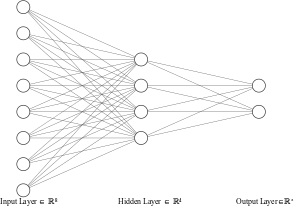
\includegraphics{Imagens/dense_layer.png}
	\caption{Bloco Dense}
	\label{fig:dense_blcok}
\end{figure}
	
\subsection{Blcoo CNN}

Bloco de CNN é aqui definido como uma convolução na dimensão temporal seguido de camadas para combater o overfitting, MaxPooling e Dropout.
Normalmente usada em processamentos de imagens, o uso de convuluções temporais é tambem por si mesmo uma ideia forte.

explicar om que e CNN
imagem

Usada tambem as ideias de attention, residual e o que eu chamei broad


\subsection{Blcoo LSTM}

O uso de LSTM para previsões é uma area comum, mas aqui é seguido através das ideas partilhas em \cite{Hewamalage2021}, e reforçado pelo uso em previsões energéticas demonstados em \cite{Costa2022}
O bloco LSTM é a aplicaçao das RNN, aqui sendo apenas definido como uma camada de LSTM.
Estes blocos mantêm dentro de si ligações a diferentes camadas temporais, e cada filtro criado, mantêm uma "memória" dos filtros passados.
Bastante utilizado em modelação de linguagem.

imagem


\section{Arquiteturas  \label{se:dados_tratamento}}

\subsection{Vanilla \label{se:dados_tratamento}}

O termo "Vanilla" aqui é aplicado para aquitecturas que apenas usam um bloco de cada, um de entrada, um principal, e um interpretativo.
Como exemplo a arquitetura de "VanillaCNN"

imagem da mesma

\subsection{Stacked \label{se:dados_tratamento}}

Stacked refere-se a "amontoado" onde se utiliza o bloco principal várias vezes em série.E apenas um bloco de  entrada e um interpretativo.
Como exemplo a arquitetura de "StackedCNN"

imagem da mesma

\subsection{MultiHead \label{se:dados_tratamento}}

Multihead é o termo para quando os blocos de entrada e principais são repetidos paralelamente, um caminho para cada atributo, ou uma outra paralelização à escolha. Sendo depois concatenadas essas camadas e passadas juntas para a camada interpretativa.
Aqui foi usado sempre a paralelização por atributos, e ao invês de fazer Mulithead no sentido de multiplas entradas, para simplicidade de programação, foi feito um paralização interna no modelo, apos a camada de entrada, onde a mesma é repetida para cada atributo.
Foi testado a diferença, e para os dados usados não havia diferenças de qualidade, mas sim em tempo de treino, logo a mais rapida foi a escolhida.
Como exemplo a arquitetura de "MultiheadCNN"

imagem da mesma

\subsection{MultiTail \label{se:dados_tratamento}}

Esta arquitectura tem o mesmo conceito que a anterior a nivel de paralelização, mas neste caso esta é feita apenas na camada interpretativa. Sendo que o resultado do bloco principal é repetido para criar a paralelização.
Neste caso foi paralelizado com o numero de tempos a prever, 24 horas, 24 objectos de saida destas modelos. 
A grande diferença desta arquitectura para a "Vanilla" que preve 24 horas, é que aqui cada hora tem o seu proprio valor de função de perda, logo o modelo como que está a treinar 24 modelos diferentes, e no caso "Vanilla" a função de perda é ùnica e é a media do erro das horas todas.
Como exemplo a arquitetura de "MultiTailCNN"

imagem da mesma

\subsection{UNET  \label{se:dados_tratamento}}

Normalmente usando em modelção de imagens, a arquitectura UNET passa por criar uma rede de expansão dos filtros, usando convoluções, e de seguida uma rede de contracção dos mesmo, até aos tamanhos pretendidos.
O bloco principal contextualmente o mesmo que o CNN.
Nas suas ligações UNET junta informação de filtros passados (não de nivel temporal mas de rede neuronal) para realçar informação já trabalhada, e assim identificar padrões de vários contextos diferentes.
É habitual tambem adicionar aos blocos principais portões de atenção, portões residuais. Estas duas tecnicas são tambem estudadas aqui.
É chamada assim pois é uma rede (NET) que forma um U na sua expansão e contracção.

Como exemplo a arquitetura de "UNET"

imagem da mesma


\section{Considerações adicionais  \label{se:dados_plus}}

Aqui e dizer que os modelos utilizados para teste sao as combinacoes deste blocos nestas aquiteturas.

Imagens de layers criadas com 
dense
http://alexlenail.me/NN-SVG/index.html